%==============================================================================
% Boundary-Enhanced Hard Prototype Generation (BE-HPG) for Few-Shot Medical
% Image Segmentation of Rare Organ Malformations.  IEEE conference (IEEEtran).
% Compiles on Overleaf (IEEEtran built in); IEEEtran.cls is also committed.
% Tables are generated by  python -m src.utils.aggregate  (paper/tab_*.tex);
% the pipeline figure by    python -m src.utils.figures.
%==============================================================================
\documentclass[conference]{IEEEtran}
\IEEEoverridecommandlockouts

\usepackage{cite}
\usepackage{amsmath,amssymb,amsfonts}
\usepackage{graphicx}
\usepackage{booktabs}
\usepackage{array}
\usepackage{multirow}
\usepackage{algorithm}
\usepackage{algpseudocode}
\usepackage{xcolor}
\usepackage{url}
\usepackage[hidelinks]{hyperref}

\graphicspath{{figures/}}
\newcommand{\repourl}{https://github.com/fyakkan/be-hpg}

\begin{document}

\title{Boundary-Enhanced Hard Prototype Generation for\\
Few-Shot Medical Image Segmentation of Rare Organ Malformations}

\author{\IEEEauthorblockN{Furkan Yakkan}
\IEEEauthorblockA{Abdullah G\"ul University, Kayseri, T\"urkiye\\
furkan.yakkan@agu.edu.tr}}

\maketitle

\begin{abstract}
Few-shot segmentation promises to learn new structures from a handful of annotated examples,
which is attractive for rare organ malformations where large labelled datasets are infeasible.
A recurring weakness of prototype-based few-shot learners is that a single global-average
prototype dilutes the diagnostically critical boundary of a small foreground region. We present
\emph{Boundary-Enhanced Hard Prototype Generation} (BE-HPG): a lightweight Vision-Transformer
backbone with a Support Self-Prediction (SSP) module that extracts a boundary band by
morphological dilation minus erosion and clusters its tokens with mini-batch $k$-means into
\emph{hard} prototypes, combined with global foreground/background prototypes and an auxiliary
boundary loss. We conduct a controlled comparison study of three methods---a Prototypical
Network, a Meta-RCNN-inspired feature-reweighting baseline, and BE-HPG---under identical
episodes on the Spleen task of the Medical Segmentation Decathlon. With a standard
largest-connected-component post-processing applied to all methods, BE-HPG attains the best
Dice ($0.930$ at 1-shot), IoU, and---notably---boundary accuracy (HD95 $2.9$\,px, ASD
$1.0$\,px), outperforming both baselines. We further analyse the boundary-loss weight and the
effect of post-processing, and we openly report the reduced compute budget and resulting
limitations. Code: \url{\repourl}.
\end{abstract}

\begin{IEEEkeywords}
few-shot learning, medical image segmentation, prototypical networks, vision transformer,
boundary loss, hard prototypes.
\end{IEEEkeywords}

%------------------------------------------------------------------------------
\section{Introduction}
Deep learning has transformed medical image analysis, but its success depends on large,
expert-annotated datasets. For rare genetic conditions and organ malformations, which affect
only minute fractions of the population, collecting thousands of annotated samples is clinically
and logistically infeasible. Few-shot segmentation offers an alternative by requiring only a
small \emph{support} set of annotated examples at inference time~\cite{snell2017prototypical,
hansen2022anomaly,roy2020squeeze}. However, medical foreground regions are typically very small
relative to a healthy background; when a class prototype is computed by global average pooling
over the support, the resulting representation is dominated by background context, blurring the
boundaries that are most informative for diagnosis. In many malformations the shape and sharpness
of the lesion contour are themselves the primary diagnostic cue, so a learner that
under-represents boundary features is poorly matched to the clinical task.

This work investigates whether concentrating representational power on boundary features
improves few-shot organ segmentation. We propose \emph{Boundary-Enhanced Hard Prototype
Generation} (BE-HPG), built on a lightweight Vision Transformer (ViT) backbone. A Support
Self-Prediction (SSP) module isolates a boundary band around the support mask and clusters the
features inside it into a compact set of \emph{hard} prototypes, which are matched against query
features by cosine similarity and refined with an auxiliary boundary loss.

Crucially, we frame this paper as a \emph{controlled comparison study} rather than an
advocacy of a single method. We implement and evaluate three approaches under identical
episodic sampling, augmentation, and hardware: (i) a Prototypical Network~\cite{snell2017prototypical},
(ii) a Meta-RCNN-inspired feature-reweighting baseline~\cite{yan2019meta} (whose adaptation we
disclose plainly in Section~\ref{sec:methods}), and (iii) the proposed BE-HPG. Our
contributions are: (1) a faithful, reproducible implementation of the three methods with a
shared evaluation harness; (2) BE-HPG, which combines SSP boundary-hard prototypes with global
prototypes and a boundary loss; and (3) an honest empirical analysis on MSD Spleen---including
the effect of the boundary-loss weight and of largest-connected-component post-processing---that
shows where the boundary-enhanced design helps and where it does not. All code and configurations
are released at \url{\repourl}.

%------------------------------------------------------------------------------
\section{Related Work}
\textbf{Few-shot learning.} Metric-based meta-learning classifies query samples by their
distance to class representations. Prototypical Networks~\cite{snell2017prototypical} compute a
class prototype as the mean support embedding and assign each query to the nearest prototype;
this idea underpins most few-shot segmentation methods. In segmentation it is realised densely by
comparing every query-pixel embedding against support-derived foreground and background
prototypes, so the quality of the prototypes directly determines the predicted mask. Most variants
differ in how prototypes are pooled or aligned; we instead ask which \emph{regions} of the support
should form the prototypes, and argue that the boundary band is the most discriminative.

\textbf{Few-shot medical segmentation.} Hansen \emph{et al.}~\cite{hansen2022anomaly} cast
few-shot medical segmentation as anomaly detection with self-supervised supervoxels, avoiding
explicit background modelling. Roy \emph{et al.}~\cite{roy2020squeeze} introduce
squeeze-and-excite guidance for volumetric organ segmentation with few annotated slices. These
works highlight the severe foreground/background imbalance of medical data, which motivates our
boundary-focused prototypes and a class-balanced training objective.

\textbf{Reweighting and detection-style adaptation.} Meta R-CNN~\cite{yan2019meta} extends
region-based detectors with class-attentive vectors that apply channel-wise soft attention to
remodel the detector head. We adapt this reweighting idea to dense segmentation as one of our
baselines (Section~\ref{sec:methods}).

\textbf{Vision transformers.} ViT~\cite{dosovitskiy2021image} shows that pure transformers model
long-range dependencies competitively with CNNs, while data-efficient variants such as
DeiT~\cite{touvron2021training} and mobile-friendly hybrids such as
MobileViT~\cite{mehta2022mobilevit} make transformers practical on a single GPU. We use
MobileViT-S as the primary BE-HPG backbone.

%------------------------------------------------------------------------------
\section{Materials and Methods}
\label{sec:methods}

\subsection{Dataset and Preprocessing}
We use the Spleen task (Task09) of the Medical Segmentation Decathlon (MSD)~\cite{simpson2019large},
a CT benchmark with $41$ annotated volumes. Each 3D volume is reoriented to a canonical
orientation and sliced along the axial axis; we keep only slices whose foreground occupies at
least $1\%$ of the pixels, yielding $711$ informative 2D slices. Each slice is intensity-clipped
to an abdominal soft-tissue window $[-125,275]$\,HU, min--max normalised to $[0,1]$, and resized
to $224\times224$ (bilinear for images, nearest for masks). To prevent leakage, volumes are split
\emph{by patient} into train/validation/test ($25/6/10$ volumes, i.e. $415/73/223$ slices) with a
fixed seed; support and query within an episode always come from different volumes. Example slices
with ground-truth overlays are shown in Fig.~\ref{fig:samples}.

\begin{figure}[t]
  \centering
  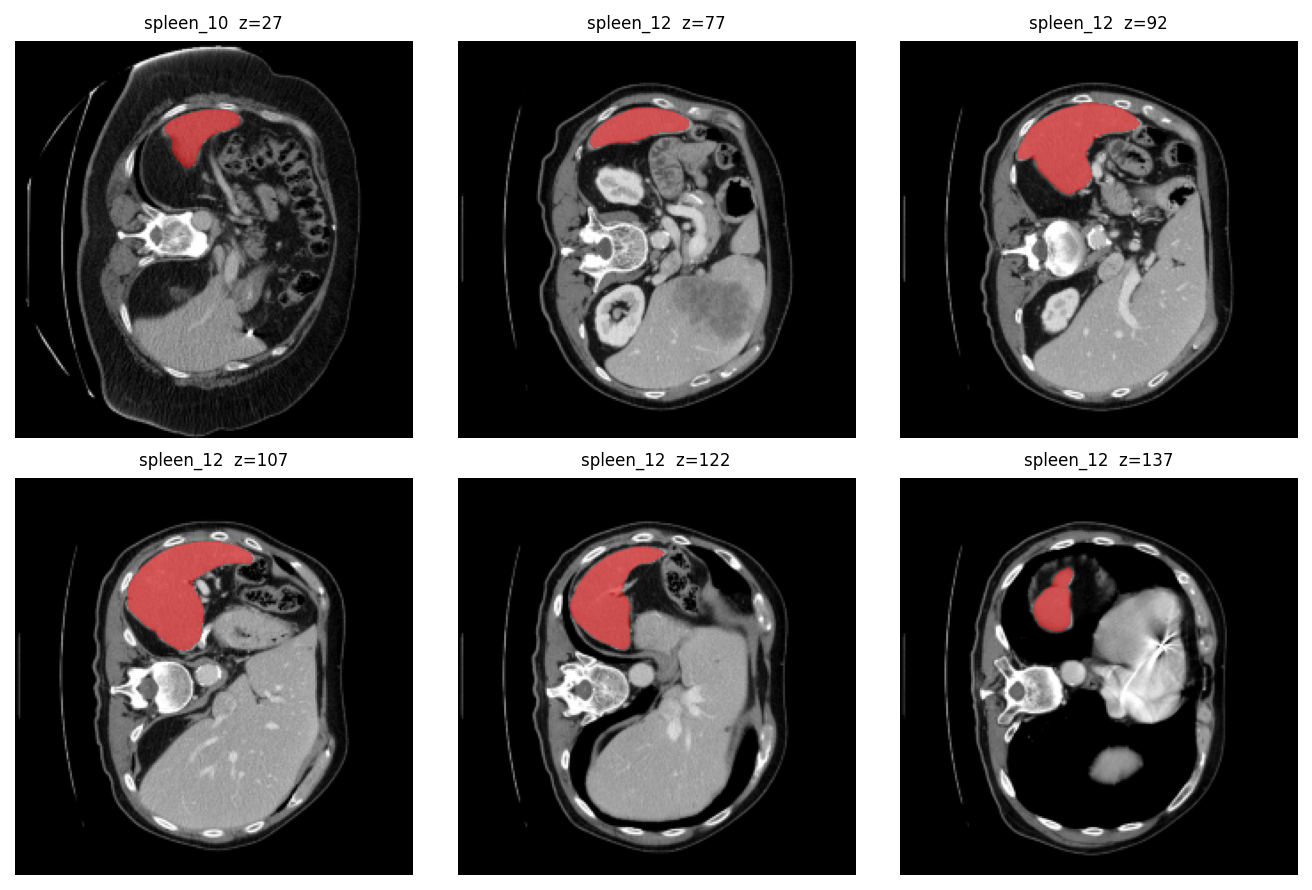
\includegraphics[width=\columnwidth]{dataset_samples.png}
  \caption{Example MSD Spleen axial slices (after HU windowing) with ground-truth spleen overlays.}
  \label{fig:samples}
\end{figure}

\subsection{Episodic Protocol}
We adopt the 1-way $K$-shot protocol: an episode comprises $K\!\in\!\{1,5\}$ support slices with
their binary masks and a small batch of query slices. To evaluate both shot settings efficiently
with a single trained model per method, $K$ is sampled per episode from $\{1,5\}$ during training
and fixed at test time. A fixed set of $150$ test episodes (seeded) is reused across all methods
for a fair comparison.

\subsection{Baseline Methods}
\textbf{Prototypical Network.} Support features $F_s$ at locations $x$ with binary mask $M_s$
yield a foreground prototype by masked global average pooling,
\begin{equation}
  p \;=\; \frac{\sum_{x} M_s(x)\,F_s(x)}{\sum_{x} M_s(x)},
  \label{eq:proto}
\end{equation}
and a background prototype analogously from $1-M_s$. A query location with feature $q$ is scored by
cosine similarity
\begin{equation}
  \mathrm{sim}(q,p) \;=\; \frac{q^{\top} p}{\lVert q\rVert\,\lVert p\rVert},
  \label{eq:cos}
\end{equation}
and the temperature-scaled difference of foreground and background similarities is passed through
a sigmoid.

\textbf{Meta-RCNN-inspired baseline (disclosed adaptation).} Meta R-CNN~\cite{yan2019meta} is a
detector; we adapt only its core idea of support-conditioned, class-attentive channel reweighting
to dense segmentation. A reweighting vector is obtained from masked support pooling
(Eq.~\ref{eq:proto}) and passed through a small MLP with a sigmoid to produce per-channel gates;
these gates modulate the query feature maps channel-wise, after which a lightweight convolutional
head ($3{\times}3$\,--\,ReLU\,--\,$1{\times}1$) predicts the mask. This is \emph{not} the original
detection architecture, and we report it as a reweighting baseline.

\subsection{Proposed Method: BE-HPG}
BE-HPG (Fig.~\ref{fig:pipeline}) passes support and query slices through a shared lightweight ViT
backbone (MobileViT-S, primary; DeiT-Tiny, secondary), producing dense token features that are
projected to a common $256$-d embedding and $\ell_2$-normalised.

\textbf{SSP hard prototypes.} At feature resolution, a boundary band is obtained as
$B=\mathrm{dilate}(M_s)-\mathrm{erode}(M_s)$, implemented with max/min pooling. The support tokens
falling inside $B$ are clustered by mini-batch $k$-means into hard prototypes $\{h_j\}_{j=1}^{k}$
that represent the discriminative transition between healthy and target tissue; an FG-interior
prototype is added from $\mathrm{erode}(M_s)$.

\textbf{Query segmentation.} For each query token $q$ we form three cosine-similarity channels---
similarity to the global foreground prototype, the maximum similarity to the hard prototypes, and
similarity to the background prototype:
\begin{equation}
  \big[\,\mathrm{sim}(q,p_{\text{fg}}),\;\; \max_{j}\,\mathrm{sim}(q,h_j),\;\; \mathrm{sim}(q,p_{\text{bg}})\,\big].
  \label{eq:channels}
\end{equation}
A $1{\times}1$ convolution followed by a sigmoid maps these channels to the mask logits, which are
bilinearly upsampled to the slice resolution. The head is initialised to the cosine-difference
prior $\tau\,(\mathrm{sim}(q,p_{\text{fg}})-\mathrm{sim}(q,p_{\text{bg}}))$, so the model starts as
a calibrated prototypical classifier and learns to add the boundary-hard signal.

\textbf{Objective.} The ground-truth boundary is obtained by a Sobel filter on the mask, and the
total loss combines a class-balanced binary cross-entropy with an auxiliary boundary term,
\begin{equation}
  \mathcal{L}_{\text{total}} \;=\; \mathcal{L}_{\text{BCE}} \;+\; \lambda\,\mathcal{L}_{\text{boundary}},
  \label{eq:total}
\end{equation}
where $\mathcal{L}_{\text{boundary}}$ is a binary cross-entropy evaluated on the Sobel boundary
pixels. The same class-balanced BCE (a per-batch foreground \texttt{pos\_weight}, capped at $20$) is
used for all three methods, which is essential to prevent the trivial all-background solution under
the strong foreground/background imbalance of abdominal CT.

\begin{algorithm}[t]
\caption{BE-HPG episode inference}
\label{alg:behpg}
\begin{algorithmic}[1]
\Require support features $F_s$, support mask $M_s$, query features $F_q$, clusters $k$
\State $p_{\text{fg}} \gets \mathrm{maskedPool}(F_s, M_s)$;\;\; $p_{\text{bg}} \gets \mathrm{maskedPool}(F_s, 1-M_s)$
\State $B \gets \mathrm{dilate}(M_s) - \mathrm{erode}(M_s)$ \Comment{boundary band}
\State $\{h_j\}_{j=1}^{k} \gets \textsc{MiniBatchKMeans}\big(\{F_s(x): x\in B\}\big)$ \Comment{hard prototypes}
\For{each query location $q \in F_q$}
  \State $c \gets [\,\mathrm{sim}(q,p_{\text{fg}}),\; \max_j \mathrm{sim}(q,h_j),\; \mathrm{sim}(q,p_{\text{bg}})\,]$
  \State $\ell(q) \gets \mathrm{Conv}_{1\times1}(c)$
\EndFor
\State \Return $\sigma(\mathrm{upsample}(\ell))$ \Comment{predicted query mask}
\end{algorithmic}
\end{algorithm}

\begin{figure}[t]
  \centering
  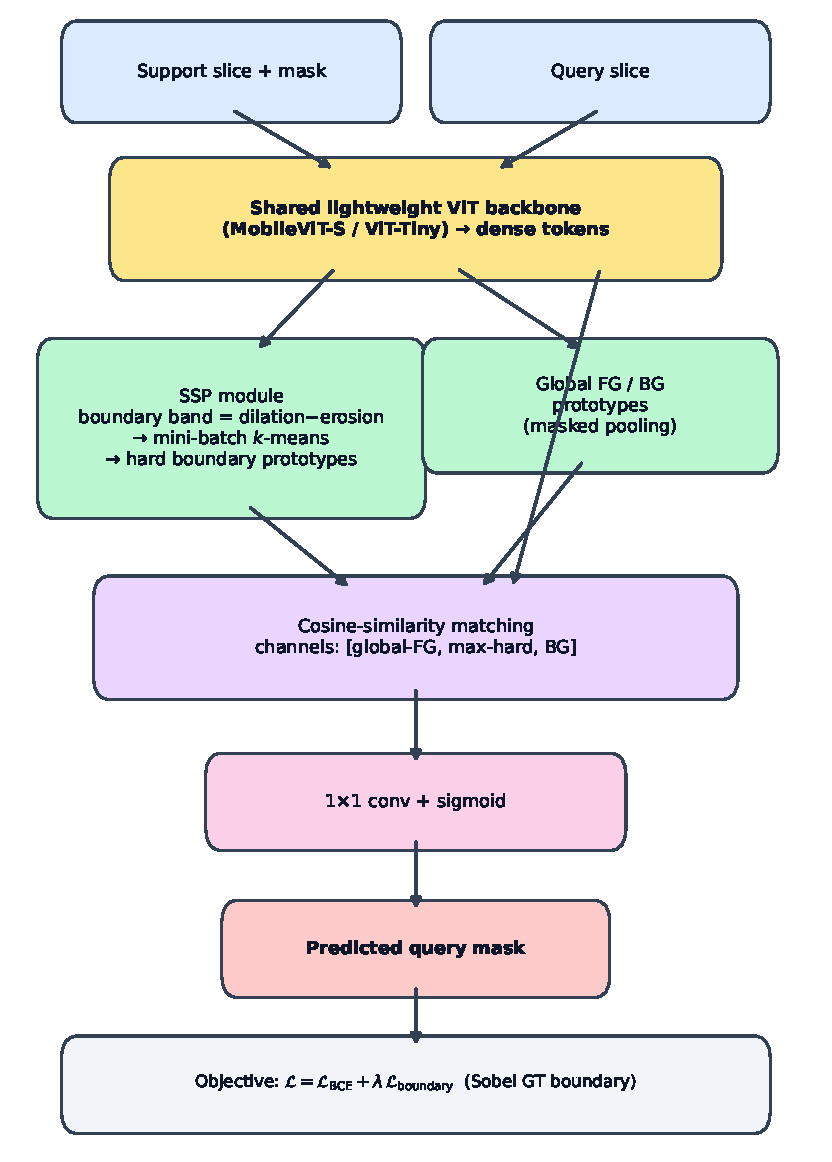
\includegraphics[width=\columnwidth]{be_hpg_pipeline.pdf}
  \caption{BE-HPG pipeline. A shared lightweight ViT backbone feeds the SSP module
  (boundary-band $k$-means hard prototypes) and the global FG/BG prototypes; three
  cosine-similarity channels are fused by a $1{\times}1$ conv head trained with
  $\mathcal{L}_{\text{BCE}}+\lambda\mathcal{L}_{\text{boundary}}$.}
  \label{fig:pipeline}
\end{figure}

%------------------------------------------------------------------------------
\section{Experimental Setup}
All methods share the same backbone projection dimension ($256$), feature stride ($8$, i.e.
$28{\times}28$ maps at $224^2$), episodic sampler, augmentation (horizontal flip, intensity
jitter), and optimiser. We use AdamW (weight decay $0.01$), learning rate $10^{-4}$ with cosine
annealing, gradient clipping at $1.0$, mixed-precision (FP16) training, and a query batch size of
$2$. The CNN baselines use a ResNet-50 backbone; BE-HPG uses MobileViT-S with $k{=}5$ hard
prototypes, a dilation kernel of $3$, and $\lambda{=}0.3$. Each method is trained for $1500$
episodes (single seed) and evaluated on the fixed $150$ test episodes at $1$- and $5$-shot.
Segmentation quality is measured by Dice and IoU; boundary quality by HD95 and ASD computed with
\texttt{medpy}, averaged only over slices where both prediction and ground truth are non-empty
(no such slices were excluded in our runs). We additionally apply largest-connected-component
(LCC) post-processing, valid for a single organ, identically to all methods.

\textbf{Scale disclosure.} Owing to a strict time budget on a single free-tier T4 GPU, this study
uses a reduced configuration relative to the original proposal: $1500$ training episodes (not
$10{,}000$), a single seed (not three), $150$ test episodes (not $500$), and the Spleen task only
(Pancreas was not run). These reductions are reflected in the limitations
(Section~\ref{sec:conclusion}); all reported numbers come from runs we executed.

\textbf{Reproducibility.} Every run is fully specified by a YAML configuration and a fixed seed.
Backbones are loaded from \texttt{timm} with ImageNet-1K pretrained weights and fine-tuned
end-to-end. The hard prototypes use scikit-learn's mini-batch $k$-means on the detached
boundary-band tokens, while the centroids used for matching are recomputed as differentiable
means of their assigned tokens, so that gradients still reach the encoder. Checkpoints are
written periodically and all runs are resumable. The data-preparation, training, and evaluation
notebooks, together with the exact configurations and a CPU test suite, are released at
\url{\repourl}.

%------------------------------------------------------------------------------
\section{Results and Discussion}

\begin{table*}[t]
\centering
\caption{Few-shot segmentation on MSD Spleen (150 test episodes, single seed), with largest-connected-component post-processing applied to all methods. HD95 and ASD are in pixels; $\downarrow$ lower is better. Best per column in \textbf{bold}.}
\label{tab:main}
\begin{tabular}{l cccc cccc}
\toprule
& \multicolumn{4}{c}{1-shot} & \multicolumn{4}{c}{5-shot} \\
\cmidrule(lr){2-5}\cmidrule(lr){6-9}
Method & Dice & IoU & HD95$\downarrow$ & ASD$\downarrow$ & Dice & IoU & HD95$\downarrow$ & ASD$\downarrow$ \\
\midrule
ProtoNet & 0.896 & 0.815 & 3.8 & 1.5 & 0.887 & 0.800 & 4.1 & 1.7 \\
Meta-RCNN-style & 0.905 & 0.830 & 3.5 & 1.4 & 0.898 & 0.819 & 4.0 & 1.4 \\
BE-HPG (ours) & \textbf{0.930} & \textbf{0.871} & \textbf{2.9} & \textbf{1.0} & \textbf{0.926} & \textbf{0.867} & \textbf{3.4} & \textbf{1.3} \\
\bottomrule
\end{tabular}
\end{table*}


\textbf{Main comparison.} Table~\ref{tab:main} reports the comparison with LCC post-processing.
All three methods segment the spleen well (Dice $\ge 0.89$), as expected for a large, well-defined
organ. BE-HPG attains the best score on \emph{every} metric at both shot settings---Dice $0.930$,
IoU $0.871$, HD95 $2.9$\,px, and ASD $1.0$\,px at $1$-shot---outperforming the Prototypical Network
and the reweighting baseline, and in particular achieving the best \emph{boundary} accuracy, which
is consistent with its boundary-enhanced design.

\textbf{Effect of shot count.} Across all three methods the $5$-shot scores are on par with, or
marginally below, the $1$-shot scores (for example BE-HPG Dice $0.930\!\rightarrow\!0.926$). On a
large, anatomically consistent organ a single support slice already yields a representative
prototype; additional support slices, drawn from a \emph{different} patient under our
volume-disjoint protocol, inject inter-patient appearance variance that can dilute the prototype
rather than sharpen it. This indicates that for such organs the bottleneck is cross-patient
generalisation rather than the number of annotated shots---a useful negative result for designing
few-shot medical pipelines.

\begin{table}[t]
\centering
\caption{1-shot HD95 (px) before/after largest-connected-component (LCC). LCC removes off-target predictions; BE-HPG benefits most, exposing its precise organ boundary.}
\label{tab:rawlcc}
\begin{tabular}{lcc}
\toprule
Method & HD95 raw & HD95 + LCC \\
\midrule
ProtoNet & 28.3 & 3.8 \\
Meta-RCNN-style & 12.8 & 3.5 \\
BE-HPG (ours) & 44.8 & 2.9 \\
\bottomrule
\end{tabular}
\end{table}


\textbf{Effect of post-processing.} Without post-processing, BE-HPG had the \emph{worst} HD95
($44.8$\,px at $1$-shot) despite a competitive Dice, because its hard-prototype matching
occasionally activates on off-target regions far from the spleen, inflating the $95$th-percentile
surface distance. Table~\ref{tab:rawlcc} shows that LCC---which simply keeps the largest predicted
component---removes these spurious activations and benefits all methods, but BE-HPG most: its raw
HD95 of $44.8$\,px drops to $2.9$\,px, the lowest of the three. In other words, the core organ
prediction of BE-HPG is the most accurate; the off-target false positives, not the boundary
localisation, were responsible for its poor raw surface metric.

\begin{table}[t]
\centering
\caption{Boundary-loss weight $\lambda$ ablation for BE-HPG on Spleen (1-shot, 1000 episodes, no post-processing). A small $\lambda$ slightly helps Dice, but HD95 worsens monotonically as $\lambda$ grows. Best in \textbf{bold}.}
\label{tab:ablation}
\begin{tabular}{ccc}
\toprule
$\lambda$ & Dice & HD95$\downarrow$ \\
\midrule
0.0 & 0.865 & \textbf{34.2} \\
0.1 & \textbf{0.874} & 44.8 \\
0.3 & 0.857 & 53.9 \\
0.5 & 0.841 & 62.0 \\
\bottomrule
\end{tabular}
\end{table}


\textbf{Boundary-loss weight.} Table~\ref{tab:ablation} ablates the boundary-loss weight
$\lambda$ (without post-processing). A small weight ($\lambda{=}0.1$) marginally improves Dice over
$\lambda{=}0$, but HD95 degrades monotonically as $\lambda$ grows ($34.2\!\to\!62.0$\,px). On a
large solid organ such as the spleen, heavy boundary emphasis therefore does not help---and can
hurt---surface accuracy; a light boundary weight is preferable. This is an honest, organ-dependent
finding: the boundary machinery is expected to pay off on thin or boundary-critical targets (the
rare malformations the method targets) rather than on large blobs.

\textbf{The role of class balancing.} The severe foreground/background imbalance of abdominal CT
makes the all-background prediction a strong local optimum for a freely parameterised
segmentation head. In preliminary runs with a plain unweighted BCE, the reweighting baseline
collapsed to predicting no foreground (Dice $\approx 0$), whereas the prototype-based methods,
whose outputs are structured cosine similarities, were unaffected. Replacing the objective with
the per-batch class-balanced BCE of Eq.~(\ref{eq:total})---applied identically to all methods---
removed this collapse and is what makes the comparison meaningful. We report this explicitly
because it is a practical prerequisite for a fair few-shot medical segmentation benchmark.

\textbf{Qualitative results.} Fig.~\ref{fig:qual} shows BE-HPG predictions on held-out query
slices; the predicted masks closely follow the ground-truth spleen contour. Fig.~\ref{fig:qual_base}
shows the two baselines on the same slices for visual comparison.

\begin{figure}[t]
  \centering
  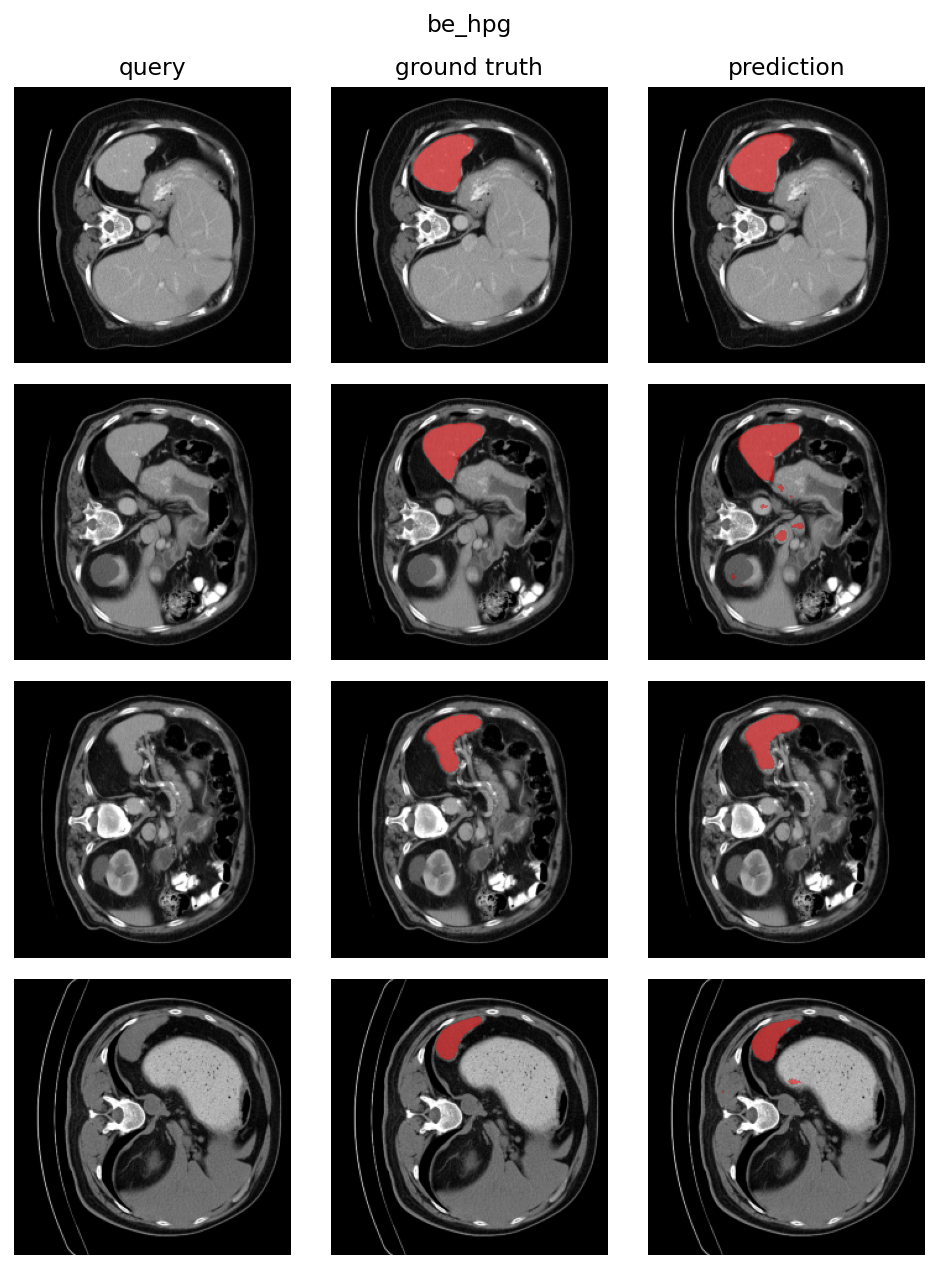
\includegraphics[width=\columnwidth]{qualitative_be_hpg.png}
  \caption{Qualitative BE-HPG results on held-out test episodes (query image, ground truth,
  prediction). Predictions track the spleen boundary closely.}
  \label{fig:qual}
\end{figure}

\begin{figure*}[t]
  \centering
  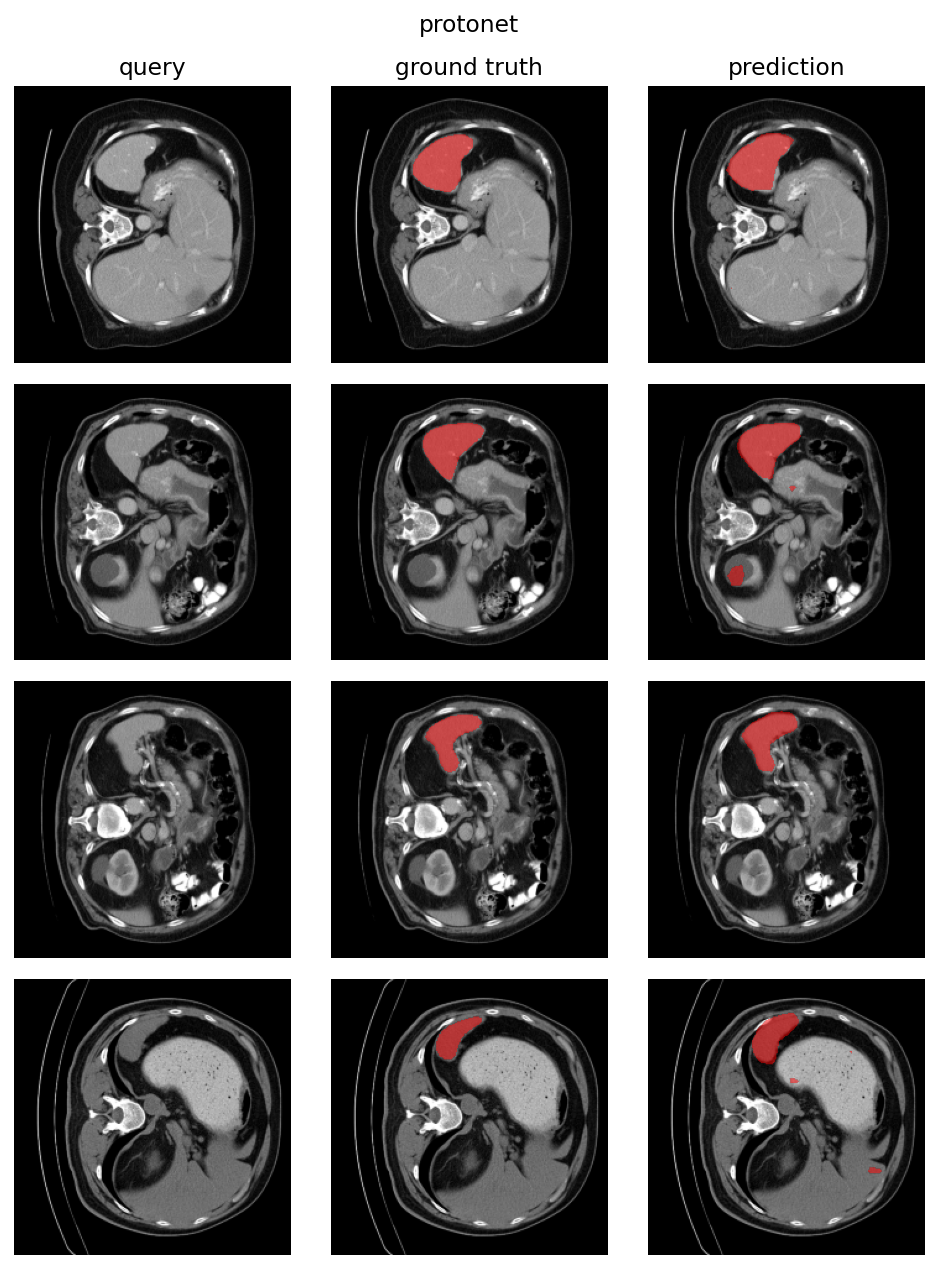
\includegraphics[height=0.32\textheight]{qualitative_protonet.png}\hfil
  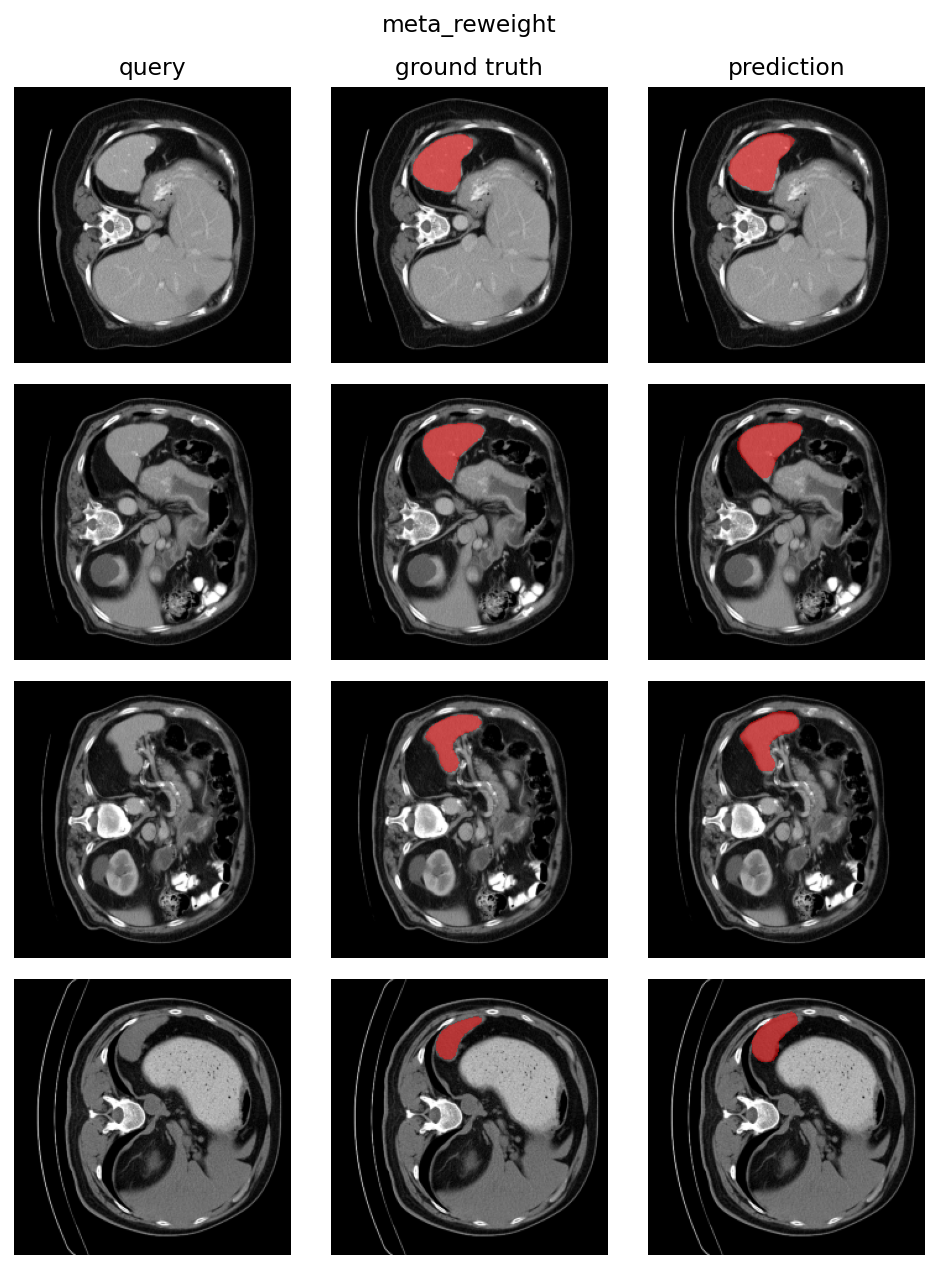
\includegraphics[height=0.32\textheight]{qualitative_meta.png}
  \caption{Qualitative baseline results on the same held-out query slices: the Prototypical
  Network (left) and the Meta-RCNN-inspired reweighting baseline (right). Each panel shows, per
  row, the query image, ground truth, and prediction. All methods segment the spleen well; the
  differences that matter on this organ are in the rare off-target activations that
  post-processing removes (Table~\ref{tab:rawlcc}).}
  \label{fig:qual_base}
\end{figure*}

%------------------------------------------------------------------------------
\section{Conclusion and Future Work}
\label{sec:conclusion}
We presented a controlled comparison of three few-shot medical segmentation methods and proposed
BE-HPG, which augments global prototypes with SSP boundary-hard prototypes and a boundary loss on a
lightweight ViT backbone. On MSD Spleen, with post-processing applied equally to all methods,
BE-HPG achieves the best overlap and boundary metrics. Our analysis also exposes two honest
caveats: BE-HPG's hard-prototype matching can produce off-target activations that a
largest-connected-component step is needed to remove, and a strong boundary-loss weight degrades
surface metrics on a large organ.

\textbf{Limitations.} The study is compute-limited: a single seed, $1500$ training and $150$ test
episodes, and a single (Spleen) task, all on a free-tier GPU. The absolute scores are therefore
single-run estimates, and the central premise---segmentation of \emph{rare malformations} with thin
or irregular boundaries---is approximated, not directly tested, by a healthy-organ benchmark.

\textbf{Future work.} Extending the evaluation to the Pancreas task, multiple seeds with confidence
intervals, the full episode budget, the DeiT-Tiny backbone and SSP-versus-global ablations, and---
most importantly---a dataset of genuine boundary-critical pathologies would more directly test the
boundary-enhanced hypothesis.

%------------------------------------------------------------------------------
\section*{Acknowledgment}
This work made use of a generative AI assistant for parts of the code implementation, experiment
orchestration, and figure and table generation. All experimental results were produced by runs the
author executed on Google Colab, and every citation was independently verified by the author, who
takes full responsibility for the correctness and integrity of this work.

%------------------------------------------------------------------------------
\bibliographystyle{IEEEtran}
\bibliography{refs}

\end{document}
